\section{Strategies for Gathering of Results}
\subsection{Chosen Metric: Accuracy}
The metric chosen for the following experiments was accuracy, due to its comprehensible nature. Despite the fact that an unbalanced dataset presents one of the significant drawbacks of using accuracy, this concern is irrelevant in the case of MNIST-F since it is a balanced dataset. The accuracy of each node is computed after each training step using the test subset of MNIST-F, and none of the nodes are ever provided access to the test set for training.

\subsection{Number of Simulated Nodes}
The experiments were conducted using 10 nodes, with the exception of the server in cases where FedAvg was employed. The decision of how many nodes to simulate was based on the highest node count attainable without causing inconsistencies and crashes due to resource depletion of the training machine.

\subsection{Repeated Testing for Noise Reduction}
The training process for each experiment was conducted five times, and the resulting accuracies of every node were recorded. To mitigate the impact of training noise on the performance graphs, the accuracy value for each time step was calculated as the median accuracy across all nodes and runs at that time step. As there were 10 nodes, this resulted in the graphs representing median of 50 nodes.

\subsection{Configuring the Algorithm}
In each of the following experiments, the algorithm was configured using a specific set of parameters $\alpha \beta \gamma$. These parameters were obtained heuristically by making an initial guess, testing, and then fine-tuning them until a satisfactory outcome was reached. However, it is important to note that an exhaustive investigation into the optimal parameter configuration for a particular type of problem is not within this papers scope, meaning that it is plausible that swarm learning could yield better results with more precisely tuned parameters.

\subsection{Data Provided to Each Node}
The experiments evaluate the algorithm's performance using three levels of data volume per node. These levels are considerably smaller than the full MNIST-F dataset not only to increase problem difficulty, but also as the algorithm is intended for scenarios where each nodes access to data is restricted. To create a subsection of data for each node, a random sampling with replacement method was used to select the desired number of datapoints. During the initial training phase, each node performs a single sampling of its dataset, after which that nodes data subset remains constant. The three levels of data volume can be seen in Table \ref{epsparams}.

\subsection{Training Steps and Epochs}
Due to the limited size of the dataset, a single node executes more than one epoch of training in each training step. The number of epochs carried out by a node per training step will be referred to as Epochs per Step (EPS). Empirical testing has indicated that both SL and FL exhibit improved performance with higher EPS, at times surpassing the gains from increasing the number of training steps. Moreover, the utilization of higher EPS was favoured due to its reduced training time, compared to increasing the number of training steps. The three levels of data volume with their respective EPS are shown in table \ref{epsparams}

\begin{table}[H]
	\centering
	\begin{tabular}{l|l}
		Dataset Size & EPS \\ \hline \hline
		1000   & 5  \\ \hline
		100   & 10  \\ \hline
		25  & 20 
	\end{tabular}
	\caption{The different levels of dataset size and EPS that were tested} \label{epsparams}
\end{table}

\section{Scenario 1: Densely Connected Network}
A crucial experiment for evaluating the performance of the SL algorithm involves assessing its performance under optimal circumstances, specifically within a network of nodes wherein each node is directly connected to every other node. In FL, the analogous topology involves direct connections between each node and the server. This comparison is significant as it facilitates a direct evaluation of the SL and FL algorithms under their respective ideal conditions.

The selection of the parameters for the SL algorithm was based on the authors prior experience in testing the algorithm. These parameters are presented in Table \ref{slparamsDNP}.
\begin{table}[H]
	\begin{tabular}{p{0.5cm}|l|p{11cm}}
		P & Value & Reason \\ \hline \hline
		$\alpha$  & 0.75  & Low enough to allow nodes to maintain a small variation but not so low that the nodes diverge indefinitely                               \\ \hline
		$\beta$   & 0.5   & Allows a small amount of nodes looking back, but high value is not needed as every node will be running at approximately the same speed. \\ \hline
		$\gamma$  & 8     & All nodes will always be connected to 9 other nodes, so higher is better. There is room for 1 node to be skipped to prevent deadlock.   
	\end{tabular}
	\caption{The chosen parameters for the SL algorithm} \label{slparamsDNP}
\end{table}

\subsection{Dense Network Results}
The following are the results obtained from the execution of the training script. Each graph displays the data for SwarmAvg in red, and FedAvg in black.

\begin{figure}[H] 
	\center{\textbf{Accuracy by Training Step for 1000 Samples}} \\
	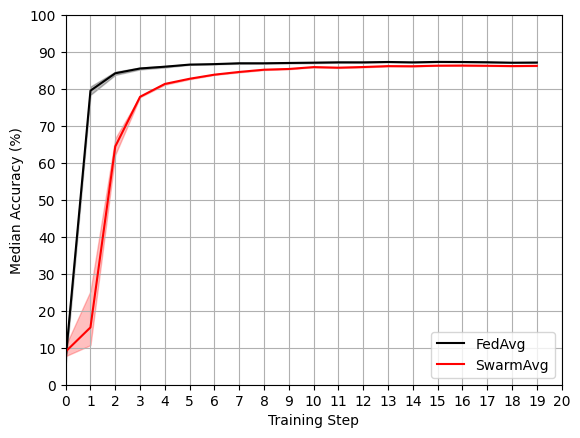
\includegraphics[width=0.49\textwidth]{aeg_dense_1000}
	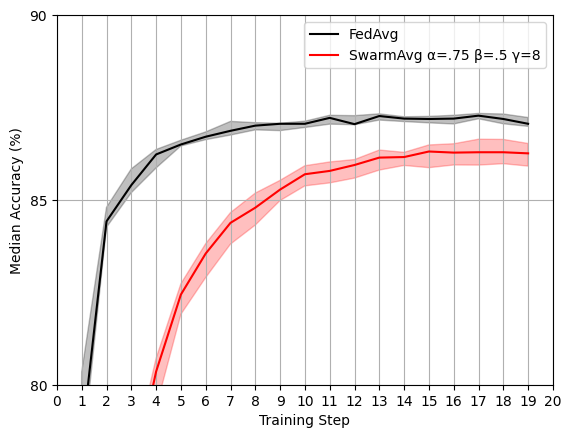
\includegraphics[width=0.49\textwidth]{aeg_dense_1000_z}
	\caption{Median accuracy by training step across 5 repeats. Each node has 1000 random data samples from MNIST-F. The shaded region surrounding each line represents the upper and lower quartile. The right-hand graph represents the same graph but zoomed in.}
	\label{aeg1}
\end{figure}

The results depicted in Figure \ref{aeg2} demonstrate that the SwarmAvg algorithm exhibits a slower convergence rate compared to FedAvg, trailing by at least 1 epoch for the duration of the test. Despite this, both methods ultimately achieve a similar level of accuracy, with less than a percent difference.

\begin{figure}[H] 
	\center{\textbf{Accuracy by Training Step for 100 Samples}} \\
	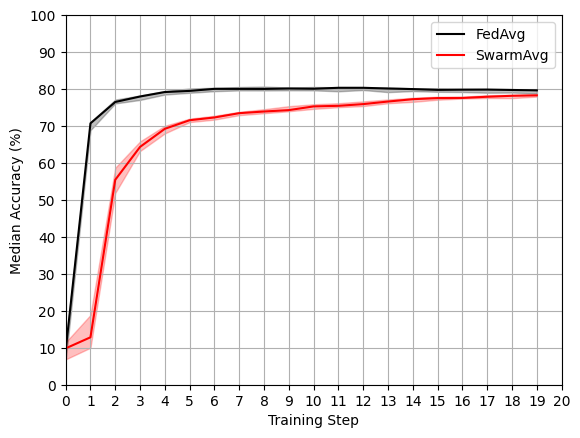
\includegraphics[width=0.49\textwidth]{aeg_dense_100}
	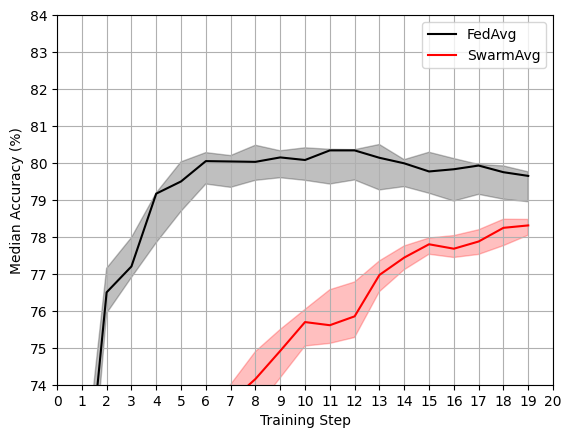
\includegraphics[width=0.49\textwidth]{aeg_dense_100_z}
	\caption{Median accuracy by training step across 5 repeats. Each node has 100 random data samples from MNIST-F. The shaded region surrounding each line represents the upper and lower quartile. The right-hand graph represents the same graph but zoomed in.}
	\label{aeg2}
\end{figure}



\begin{figure}[H] 
	\center{\textbf{Accuracy by Training Step for 25 Samples}} \\
	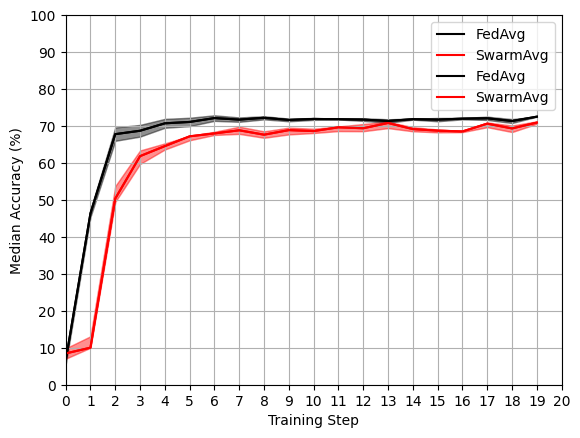
\includegraphics[width=0.49\textwidth]{aeg_dense_25}
	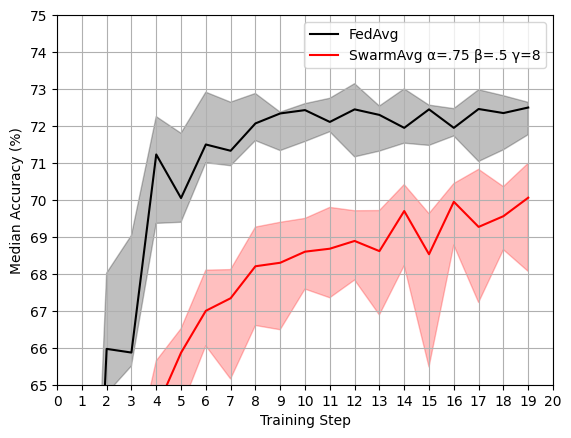
\includegraphics[width=0.49\textwidth]{aeg_dense_25_z}
	\caption{Median accuracy by training step across 5 repeats. Each node has 25 random data samples from MNIST-F. The shaded region surrounding each line represents the upper and lower quartile. The right-hand graph represents the same graph but zoomed in.}
	\label{aeg3}
\end{figure}

The trend of SwarmAvg ending with a lower accuracy than FedAvg continues in Figure \ref{aeg3}. Both algorithms also have a much lower accuracy than what they achieved previously, due to the drastic decrease in available data.

Similarly to Figure \ref{aeg2}, Figure \ref{aeg3} shows that SwarmAvg concludes with a lower accuracy than FedAvg. Furthermore, both algorithms exhibit a considerable decline in accuracy when compared to their previous performances with higher volumes of data.

\subsection{Analysis of Dense Network}

The most noticeable impact resulting from reducing the volume of data is the significant decrease in the accuracy of both algorithms, as expected. However, it is also evident that the reduction in data affects SwarmAvg and FedAvg to a similar degree, as both of their peak accuracies stay within a similar range of each other in all tests. The difference in peak accuracy between the two algorithms was quite small, often within a 2 percent margin.

One of the prominent challenges associated with SwarmAvg is its slower convergence rate compared to FedAvg, particularly from the outset. SwarmAvg consistently takes a longer time to attain its peak accuracy. This may be attributed to the asynchronous nature of the nodes in SwarmAvg, which implies that some nodes that conduct training before others may have lower accuracy than expected.

It is worth noting that in all these evaluations, SwarmAvg has a slightly higher inter-quartile range than FedAvg, indicating that FedAvg is more consistent in terms of accuracy. However, this difference is minor.

One interesting feature of both SwarmAvg and FedAvg is that both algorithms seem to be affected by overfitting much less what would be expected. Especially with just 25 data samples per node, the effects of overfitting would usually be far more severe in a single node. However, this does not mean that the algorithms do not overfit, but it may indicate that the process of overfitting for them is drastically slowed down.

\section{Scenario 2: Sparsely Connected Network}
In reality, it is uncommon for each node to be linked with every other node. To simulate a more realistic scenario, a technique was employed to generate a network of nodes with a specific density. It is important to note that, moving forward, density refers to an artificial metric and is not associated with the physical definition of density. When density is set to 0, the network is minimally linked, meaning that each node has at least one indirect path to every other node, but the minimal number of connections required to accomplish this exist. When density is set to 1, all nodes are connected to one another in a dense fashion. Since this measure may not provide a straightforward indicator of network density, two additional metrics will be provided:  Mean Minimum Hops (MMH) and Mean Connections per Node (MCPN). MMH denotes the mean minimum number of transitions required to get from one node to another in the network. MCPN denotes the average number of connections a given node possess, for a network of 10 nodes.

In order to conduct thorough testing on a variety of potential deployment scenarios, several different densities were tested for each count of data. The densities that were tested, along with their corresponding MMH and MCPN, are presented in Table \ref{sparsedensities}.

\begin{table}[H]
	\centering
	\begin{tabular}{l|l|l}
		Density & MMH & MCPN \\ \hline
		1 & 1.0 & 9.0 \\
		0.75    & 1.2 & 7.2  \\
		0.5    & 1.4 & 5.4  \\
		0.25    & 1.7 & 3.6  \\
		0    & 3.0 & 1.8  \\
	\end{tabular}
	\caption{The statistics for different density levels} \label{sparsedensities}
\end{table}

In order to assist the reader with visualizing the various density levels, some sample networks that were generated for each density can be found in Figure \ref{densefig}.

\begin{figure}[H]
	\centering
	\begin{subfigure}[b]{0.3\textwidth}
		\centering
		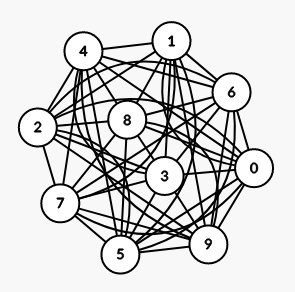
\includegraphics[width=\textwidth]{sparsegraph100}
		\caption{$density=1.0$}
	\end{subfigure}
	\begin{subfigure}[b]{0.3\textwidth}
		\centering
		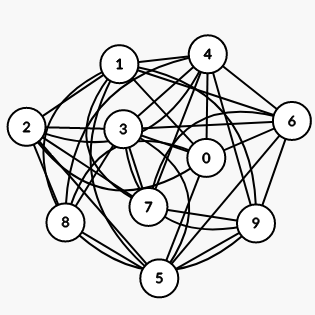
\includegraphics[width=\textwidth]{sparsegraph75}
		\caption{$density=0.75$}
	\end{subfigure}
	\begin{subfigure}[b]{0.3\textwidth}
		\centering
		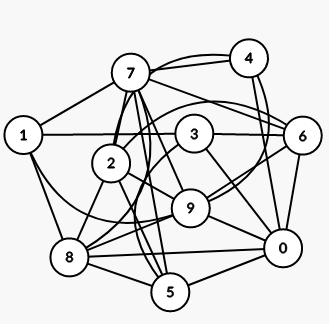
\includegraphics[width=\textwidth]{sparsegraph50}
		\caption{$density=0.5$}
	\end{subfigure}
	\begin{subfigure}[b]{0.3\textwidth}
		\centering
		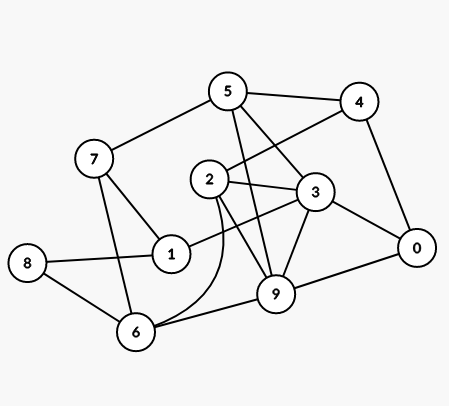
\includegraphics[width=\textwidth]{sparsegraph25}
		\caption{$density=0.25$}
	\end{subfigure}
	\begin{subfigure}[b]{0.3\textwidth}
		\centering
		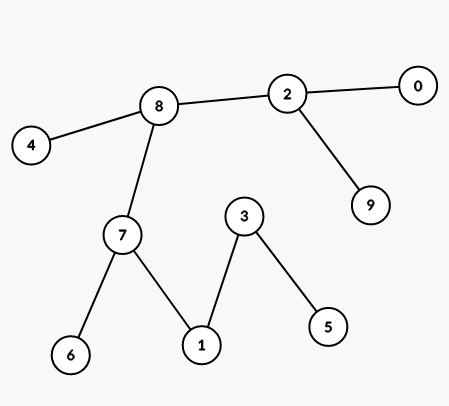
\includegraphics[width=\textwidth]{sparsegraph0}
		\caption{$density=0.0$}
	\end{subfigure}
	\caption{Example networks of nodes generated for each density level, visualised using the tool at \emph{https://csacademy.com/app/graph\_editor}. Each time a simulation is started, a new random network is generated for that simulation. \label{densefig}}
{}\end{figure}


This section does not include any testing of FedAvg. In scenarios where not every node is directly connected to the server node, FedAvg has two potential options: ignore all nodes which are not directly connected, or attempt to relay the model updates through connected nodes. As mentioned in Section \ref{relay}, relaying may not always be the optimal solution. Ignoring nodes is also not a good option, as data is wasted. Therefore, in this test, the decision was made to solely evaluate SwarmAvg.


\subsection{Sparse Network Results}
Presented below are the results obtained from executing the testing script. The density of each line on the graph is indicated by the colour, with a green hue representing higher density and a red hue indicating lower density. For all tested densities, the value of $\gamma$ was set to $round_{down}(MCPN) - 1$, which ensures that each node can progress only after waiting for all but one of its neighbours. Notably, failure to reduce $\gamma$ for less dense networks would cause several nodes to wait for a number of neighbours that cannot be achieved. Due to the random nature of the graph generation, there will still be some nodes who do not have $\gamma$ neighbours, but this should be rare and the loop to wait for $\gamma$ neighbours will terminate after a certain number of tries anyway, ensuring that training can progress.

\begin{figure}[H] 
	\center{\textbf{Accuracy by Training Step for 1000 Samples}} \\
	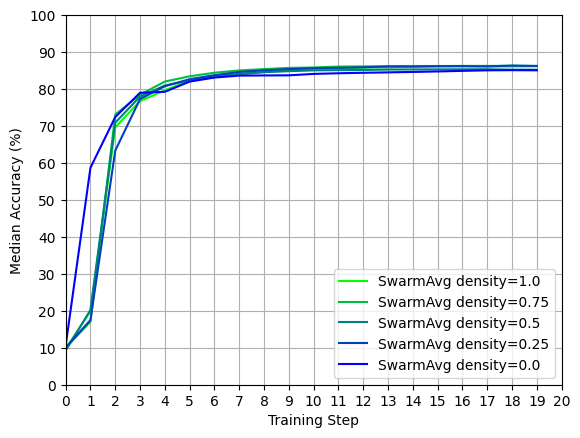
\includegraphics[width=0.49\textwidth]{aeg_sparse_1000}
	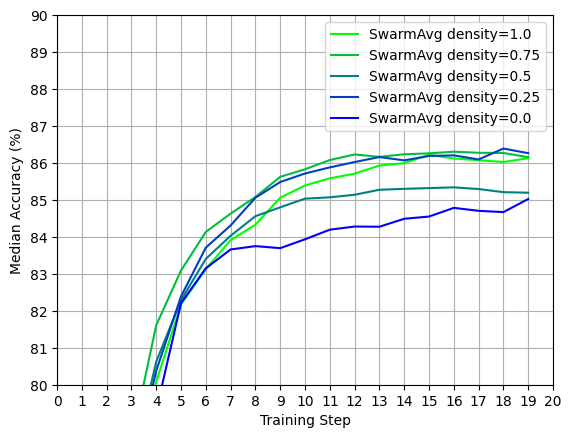
\includegraphics[width=0.49\textwidth]{aeg_sparse_1000_z}
	\caption{Median accuracy by training step across 5 repeats. Each node has 1000 random data samples from MNIST-F. Quartiles are not shown. The right-hand graph represents the same graph but zoomed in. The more green a line is, the higher its density}
	\label{aeg4}
\end{figure}

An observation that can be made of Figure \ref{aeg4} is that the different network densities perform very similarly. The final accuracy for all of the tests fell within a 2 percent range,  with the higher densities occupying the higher end.

One interesting feature of the Figure \ref{aeg4} is that the lowest density demonstrates faster convergence initially that the other densities. The author hypothesises that this may be due to groups of nodes forming local sub-networks which converge on their own sub-sets of data faster, but more slowly combine into the network as a whole as training progresses.

\begin{figure}[H] 
	\center{\textbf{Accuracy by Training Step for 100 Samples}} \\
	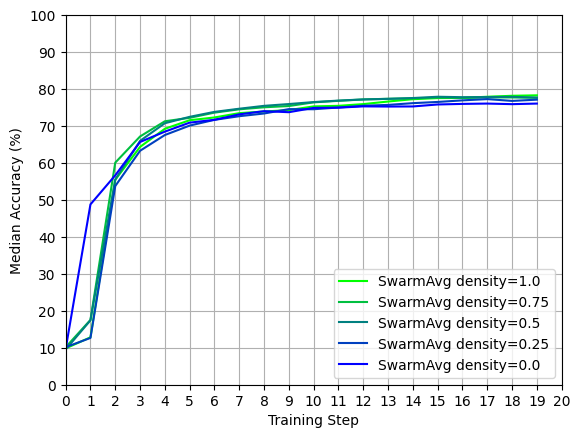
\includegraphics[width=0.49\textwidth]{aeg_sparse_100}
	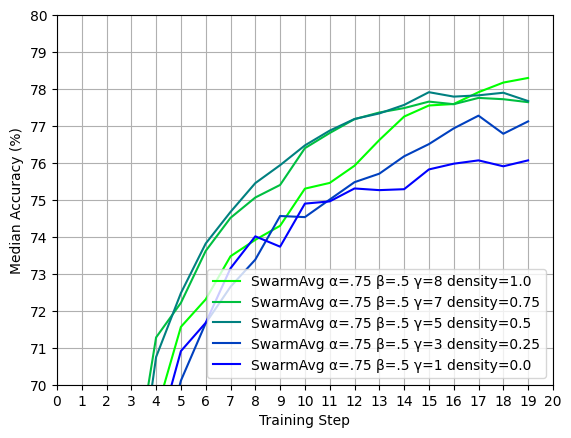
\includegraphics[width=0.49\textwidth]{aeg_sparse_100_z}
	\caption{Median accuracy by training step across 5 repeats. Each node has 100 random data samples from MNIST-F. Quartiles are not shown. The right-hand graph represents the same graph but zoomed in. The more green a line is, the higher its density}
	\label{aeg5}
\end{figure}

In Figure \ref{aeg5}, there is a slightly greater spread of final accuracies than is shown in Figure \ref{aeg4}. However, the difference is marginal. The more noticeable feature of Figure \ref{aeg5} is that the final accuracies of all densities are approximately 8 percent lower than their counterparts with more data available in figure \ref{aeg4}.

\begin{figure}[H] 
	\center{\textbf{Accuracy by Training Step for 25 Samples}} \\
	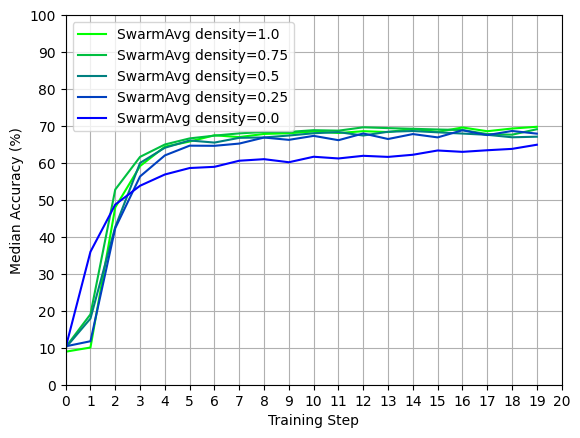
\includegraphics[width=0.49\textwidth]{aeg_sparse_25}
	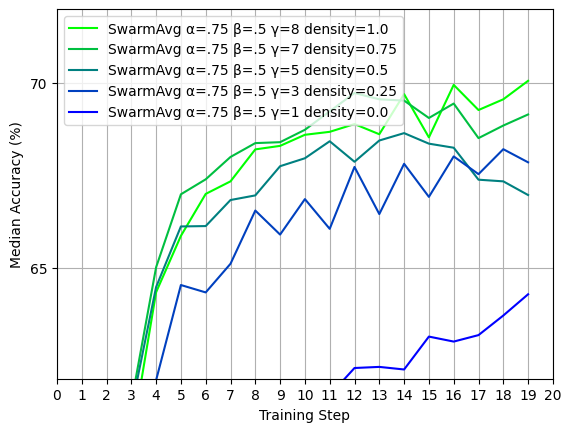
\includegraphics[width=0.49\textwidth]{aeg_sparse_25_z}
	\caption{Median accuracy by training step across 5 repeats. Each node has 25 random data samples from MNIST-F. Quartiles are not shown. The right-hand graph represents the same graph but zoomed in. The more green a line is, the higher its density}
	\label{aeg6}
\end{figure}

With just 25 data samples, the tests depicted in Figure \ref{aeg6} show a much higher variation in final accuracies than the previous two figures. There is also a much higher degree of noise in this figure than any other, suggesting that training may be much less stable with this small number of data samples to train on.

It should also be noted that the lowest density is still exhibiting the behaviour of outperforming the other densities in the initial steps, however it appears that this effect has become slightly less prominent.

\subsection{Analysis of Sparse Network}
In general, altering the network density of nodes has a small impact on the training of the nodes within the network. Decreasing the density of nodes typically leads to a lower final accuracy. This effect becomes more noticeable as the data volume provided to each node decreases, as demonstrated by the increased variability in training displayed in Figure \ref{aeg6} in comparison to Figures \ref{aeg4} and \ref{aeg5}.

The networks possessing a density of 0 attain their optima at a faster rate than those with higher densities. Figure \ref{aeg6} illustrates that the lower densities reach convergence marginally quicker than higher densities, yet are surpassed by the latter towards the end of training.

\section{Scenario 3: Densely Connected Network with Class Restrictions}

\begin{itemize}
	\item Test with each node only getting access to three classes
	\item Test both FL and SL
	\item Test on different levels of data
\end{itemize}